\section{Introduction} \label{sec:intro}
%
%\subsection{Prepare for meeting}
%formulate problem
% why cache?
%\begin{itemize}
%\item less computational load
%\item faster response time
%\item better use of bandwidth \ref{sec:intro}
%\item
%\end{itemize}
%
%Describe strait forward solution
%
%just store query results in cache and only consider direct cache hit with a
%simple cache policy like LRU or even FIFO
%
%
%Come up with some simple solutions
%
%prepare:
%\begin{itemize}
%\item The definition and problem setting of shortest path caching
%\item Some simple methods
%\item Running examples to show how these methods work
%\item Identify advantages / disadvantages of these methods
%\end{itemize}


\section{Problem}

\subsection{Definitions and problem setting}
We assume a setting where owners of mobile, positioning enabled, devices want route planning assistance. We assume users prefer online route planning services over offline solutions. 
we expect users to use network enabled capable of determining and visualizing users location and route.
Users want fast response times from online services, comparable to using an offline application \cite{ref}
Using a cache reduces the computational burden \cite{ref} on an online service, providing faster end-user response time \cite{ref} by both freeing up computational resources to calculate new routes, as well as being able to immediately provide the shortest  path result from the cache.
We assume a scenario using only server side caching.


\subsection{model}
We use a uniform random model(URM) together with a simple 'map',the graph in figure \ref{fig:simplemap}, enable us to clearly argue about the advantages expected when using server side caching of shortest-path queries. By using the simple map (fig.\ref{fig:simplemap}) and a URM together with we can reason about the probabilities that a specific query will occur. Figure \ref{fig:queryprob} illustrates the number of queries possible for a map with 2,3, and 5 locations for figure \ref{fig:queryprob}A, \ref{fig:queryprob}B, and \ref{fig:queryprob}C respectively. Each line underneeth each of the simple graphs represents two possible queries (A->B, B<-A). The number of shortest-path queries possible on a tree-graph with n vertices is n*(n-1). The probability of seeing any one query, $q_i$ is then $P(q_i | n) = (n*n-1)^{-1}$



%assume uniform random model
%use simple map
%probability of specific query is nodes*nodes-1

\begin{figure}
  \center
	\includegraphics[width=0.25\textwidth]{figures/simplemap.pdf}
	\caption{Simple map}
  \label{fig:simplemap}
\end{figure}

\begin{figure}
  \center
	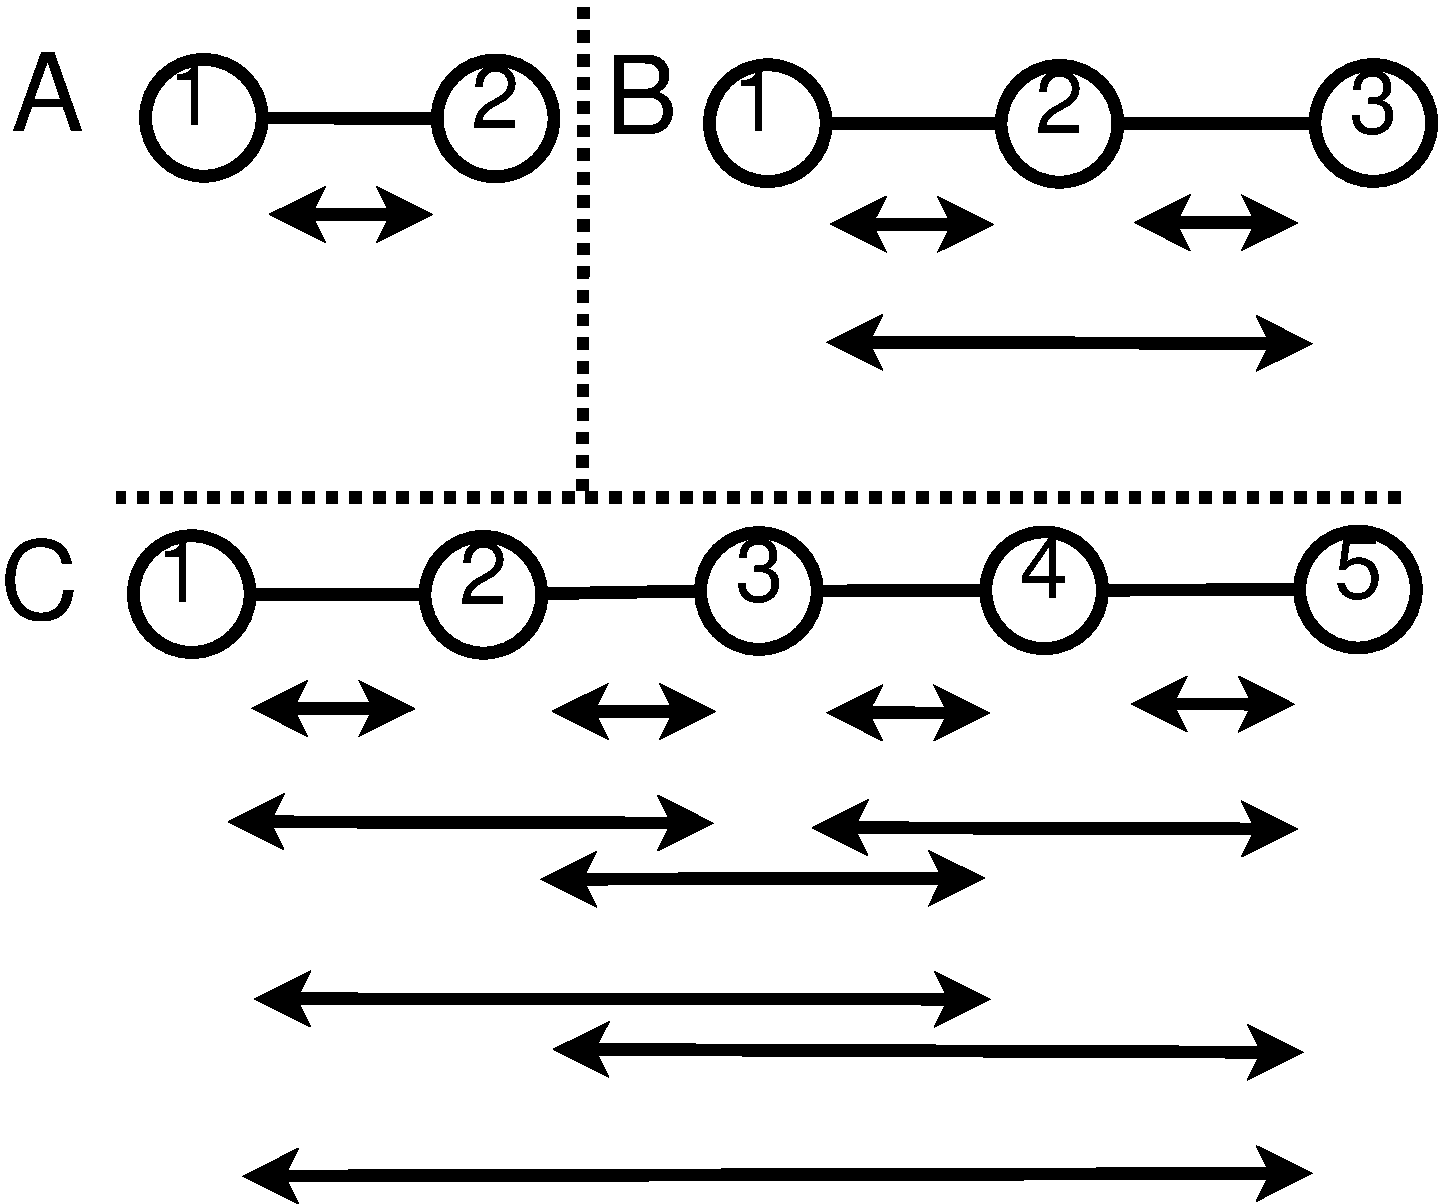
\includegraphics[width=0.25\textwidth]{figures/queryprob.pdf}
	\caption{Simple map}
  \label{fig:queryprob}
\end{figure}

\subsection{methods}

For the sake of simplicity the methods presented in this section will all be based on figure \ref{fig:simplemap} and \ref{fig:simpleroutequery}. Figure \ref{fig:simplemap} shows a simple graph which we will use as our map and figure \ref{fig:simpleroutequery} shows the simple scenario in which a user (fig. \ref{fig:simplemap}A) issues a route-planning query from 1 to 4 (fig. \ref{fig:simplemap})  to an online route-planning server with a build in cache (fig. \ref{fig:simplemap}B).


\subsubsection{Baseline}\label{baselinemethod}
The strait forward baseline solution is illustrated in figure \ref{fig:simpleroutequery}B. The idea is a server side shortest path cache which will store each query result in the cache and only consider exact query matches as cache hits, and to only use a simple cache policy such as LRU or FIFO.
The advantage of this solution is clear: it is simple and easily implemented. 
This simplicity is however obviously also it's main disadvantage, as it is too simple and very inefficient in terms of the utility the cache provides. Using items in the cache only when there is an exact match makes it exceedingly unlikely to get a cache hit due to the nature of route planning (many people share parts of routes, but few the same start and end points) and the sheer number of start-/end-point combinations possible.

\begin{figure}
  \center
	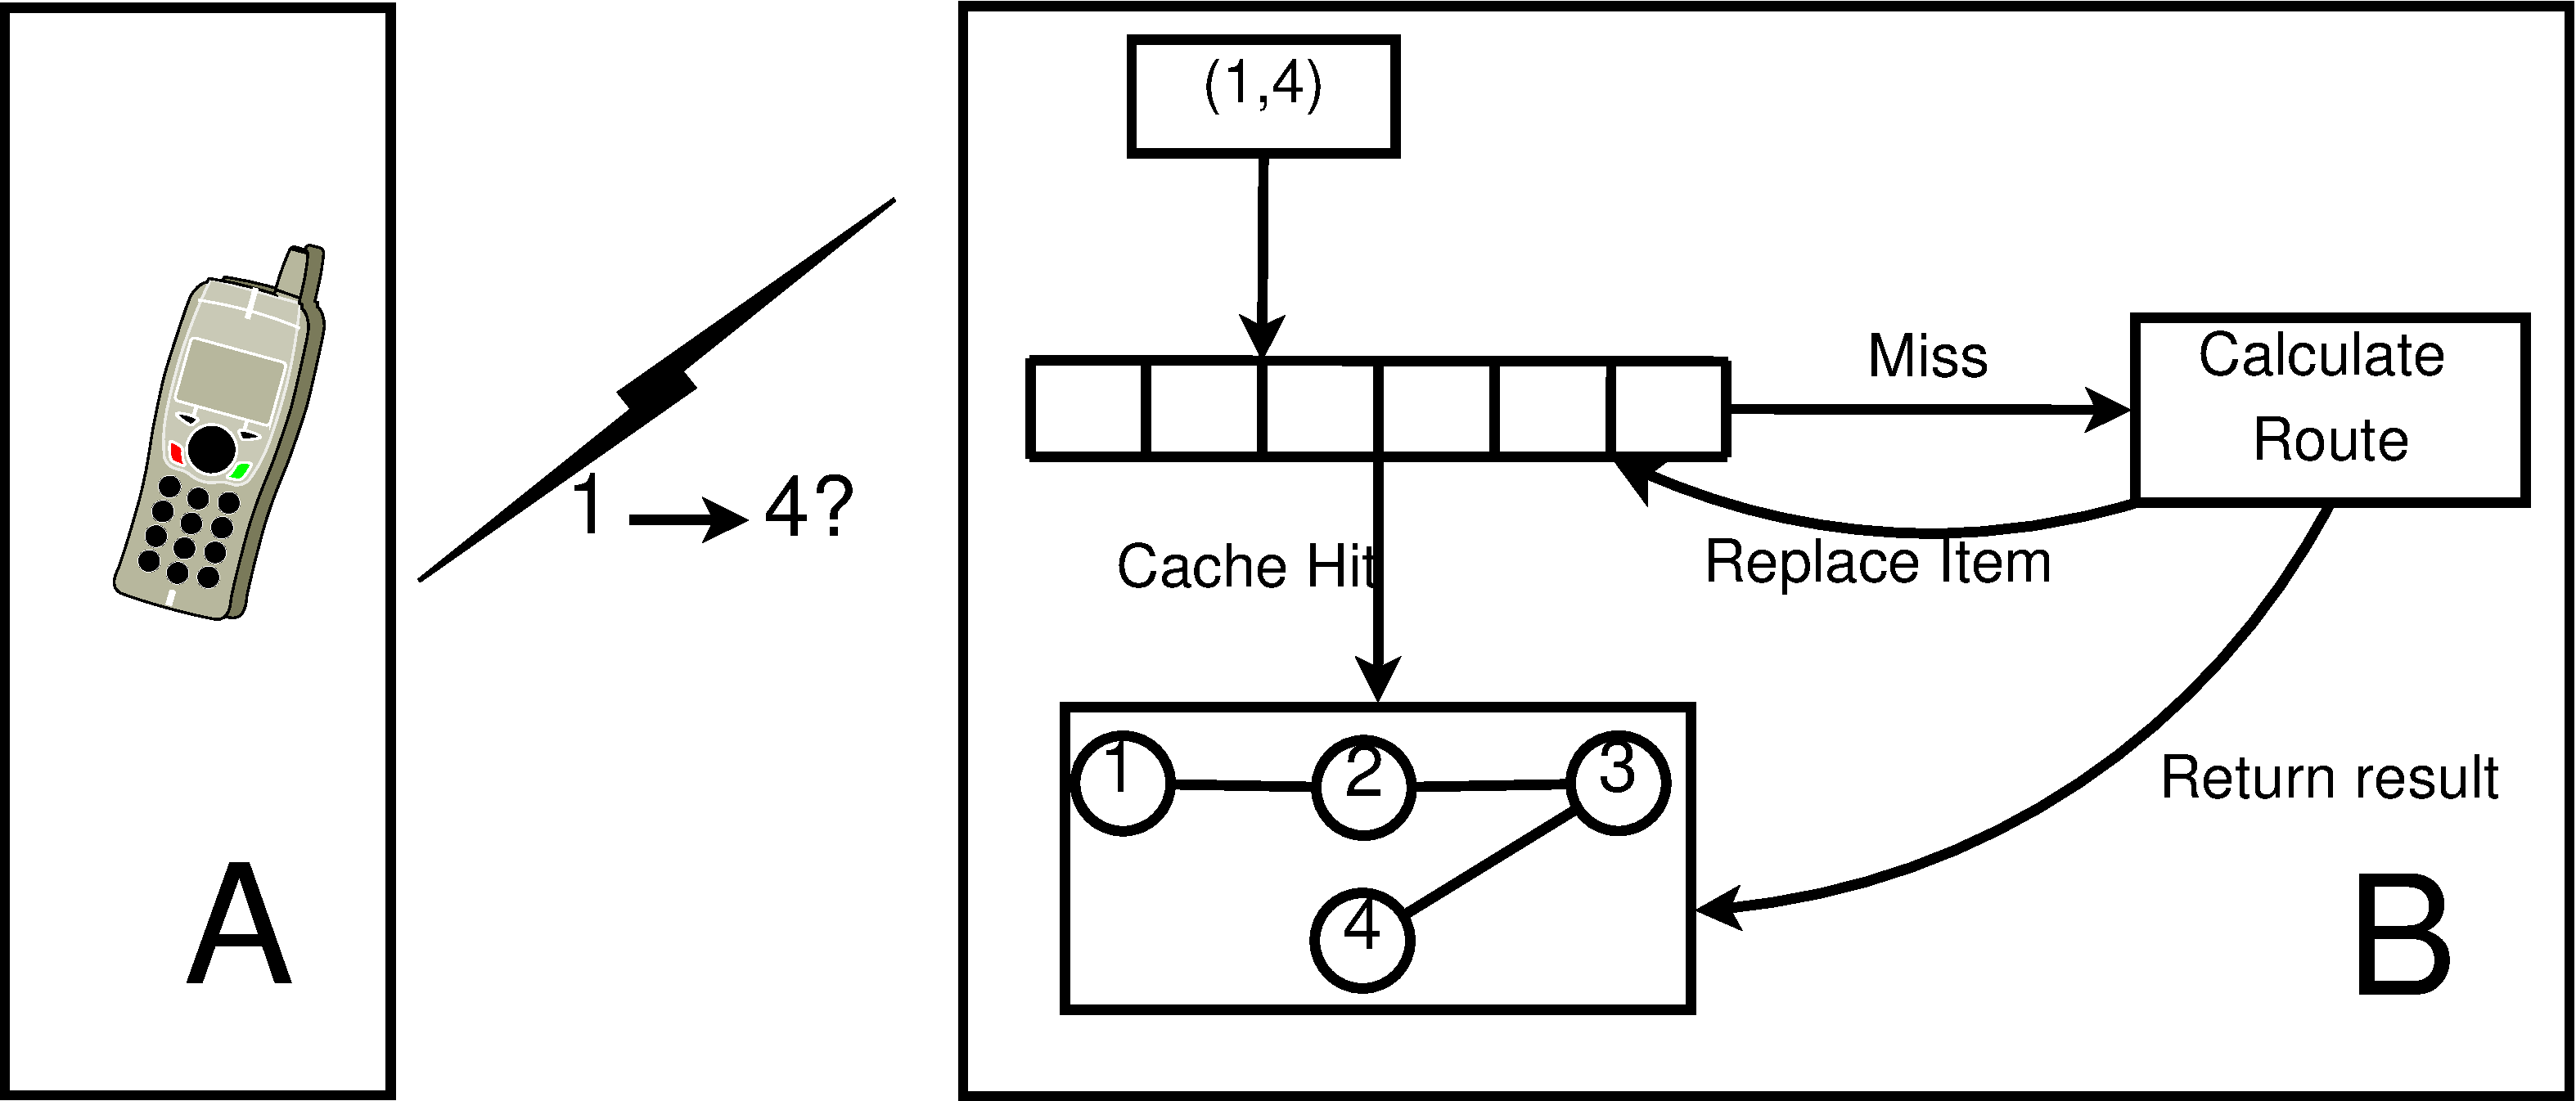
\includegraphics[width=0.5\textwidth]{figures/simpleroutequery.pdf}
	\caption{simple graph}
  \label{fig:simpleroutequery}
\end{figure}

\subsubsection{ImpBaseline}\label{baselinemethodimp}
One way to possible increase the utility of a naive cache as proposed in \ref{baselinemethod} would be to exploit the optimal substructure property\cite{introalg} of the cache items.
There is a significant increase in cache hits to be expected by utilizing the optimal substructure of shortest path cache items since it is unlikely many people will plan a route from/to the same place, but it is very likely that some sub-parts will be shared among users, and some users' full path laying within a longer path already calculated. The idea is illustrated in figure \ref{fig:cacheQueries} where the baseline method would be able to answer query Q1 from the cache, but not Q2. It is this specific disadvange which ImpBaseline addresses and ImpBaseline can therefor answer both Q1 and Q2 from the cache since the result of Q2 now exist as a solution to a subpath of cache item C3.
The disadvantage of doing this is the aditional computational resources required to examine the substructure of each  cached shortest path search result. It is currently not known if doing this is worth the efford, compaired to just calculating the route, possibly multiple times.

\begin{figure}
  \center
	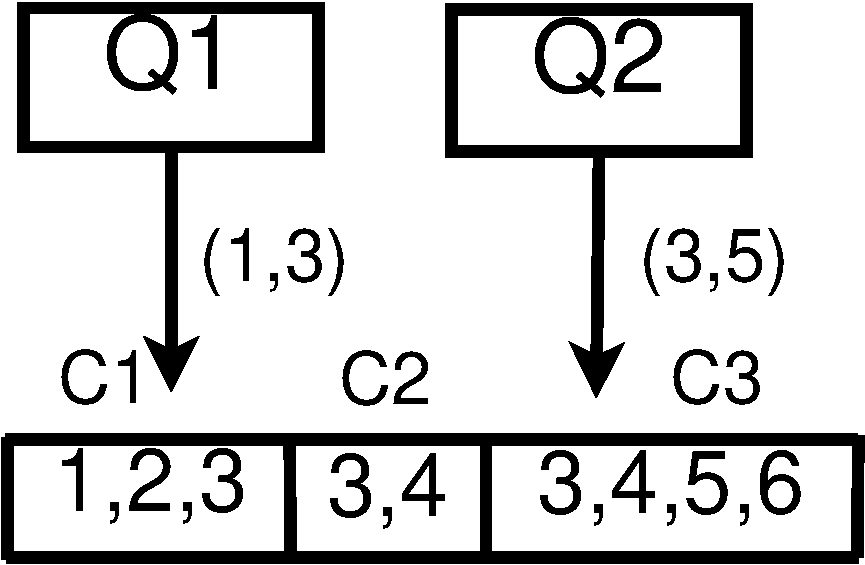
\includegraphics[width=0.25\textwidth]{figures/cacheQueries.pdf}
	\caption{Queries}
  \label{fig:cacheQueries}
\end{figure}

\subsubsection{OSC}%optimal substructure cache
OSC is more advanced than the two previous proposed solutions and therefor the scenario has been updated in figure \ref{fig:advancedroutequery}. 
To further improve upon ImpBaseline we will again utilize the optimal substructure, making it possible to have much fewer items in cache and still retain a high cache hit percentage \cite{ref}. %(assumption, need test result or proof), 
Results with sub-paths shared by many users and longer, rather than short, paths are prefered to increase the utility of the cached shortest-path results.

By adding a more intuitive cache replacement policy which takes in to consideration both the usage of each cache item, as well as the coverage of previously often seen queries it is likely that the utility of the cache would be much higher. This addition is shown with the addition of the "`add to cache"' box in figure \ref{fig:advancedroutequery}B, added to show a huristic\footnote{the actual huristic will ofcause only be defined later} will be used instead of a very simple method like LRU.


%\paragraph{\textbf{Number 3, ideas}}
%use optimal substructure\\
%prefer having longer paths in cache\\
%prefer having paths with subpaths shared by many users\\
%look at utility of cache items, not just usage when designing cache replacement policy.\\
%\begin{itemize}
%\item	prefer often used cache items
%\item	prefer items which cover routes/areas often used in previous queries
%\end{itemize}


\begin{figure}
  \center
	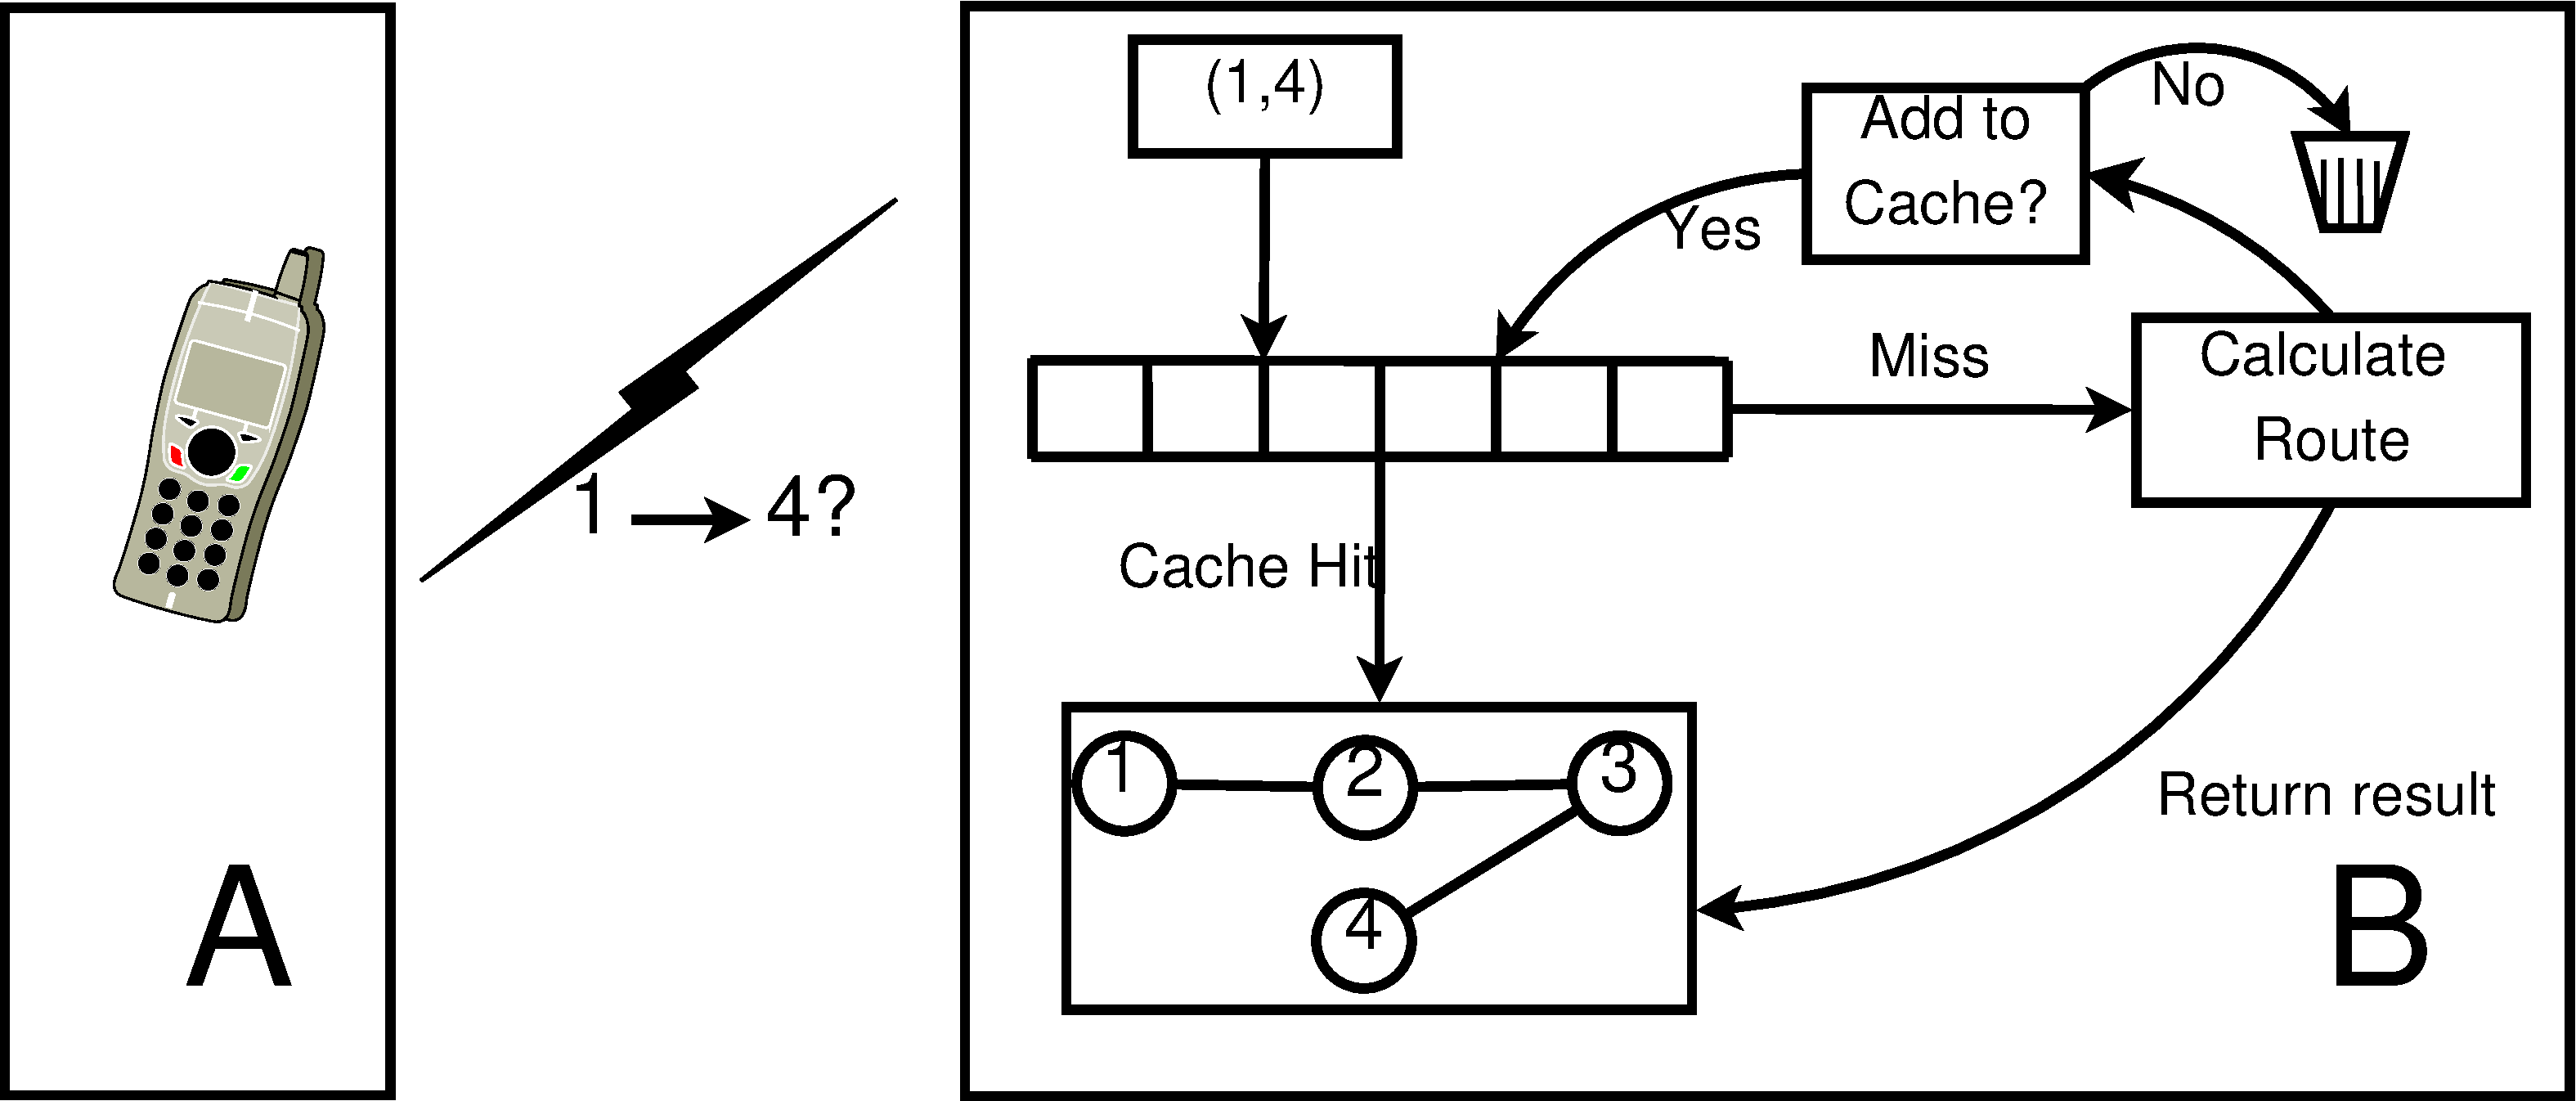
\includegraphics[width=0.5\textwidth]{figures/advancedroutequery.pdf}
	\caption{Advanced graph}
  \label{fig:advancedroutequery}
\end{figure}



%\paragraph{crap}
%We assume a setting where all users are equipped
%with a Mobile Device (MD) able to communicate and
%report the users position. All MDs are online and are
%continuesly reporting the users location at predetermined
%intervals. We use the terms user, mobile device, and
%client interchangeable and denote the set of MDs by
%UN. We expect a MD to be cabable of visualizing
%its current location.
%We assume a 2D scenario, where the movements of
%users uU are restricted to a road network G(V, E).
%V is the set of vertices, where each vertice v ∈ V
%represents either a street intersection or an important
%landmark. E is the set of directed edges augmented
%by edge length and type. Edges are represented by
%a begin/end vertice pair and each edge represents the
%smallest unit of a road segment. e ∈ E, each e being
%a tuple specifying id, start-/end-vertices, length, and
%Road Type (RT) (eid , vs , ve , elength , eRT ). RT is a
%hierarchy of the size/type of road i.e. highway, paved,
%or dirt road (Sec. 5.2).
%The simplest form of trajectory is a collection of tu-
%ples (time, longitude, latitude), ordered by the time
%attribute, but as we will work on a road network and
%in the spatio-temporal domain, such a basic notion of
%trajectories is not appropriate. We de�ne T as the set
%of trajectories, where each trajectory consist of an id
%(tid ), and a sequence of tuples containing an edge and



